\begin{DensePanel}{260mm}{3}{BEYOND NODAL: NEVER PURE DAMPING}
  {\DenseBody Keep the generator speeds $\nu$, eliminate the rest. The damping the grid supplies at frequency $\Omega$ is the Hermitian part of a full matrix, not a list of nodal coefficients:\par}
  {\DenseEq\color{IASBlue}\[
    Z=M\big(\Delta_{\nu\nu}-\Delta_{\nu h}\Delta_{hh}^{-1}\Delta_{h\nu}\big),\qquad D_H=\tfrac12\big(Z+Z^{H}\big)
  \]}
  \vspace{-2mm}
  {\DenseBody One PLL change gives a rank-two increment with one positive and one negative eigenvalue:\par}
  {\DenseEq\color{IASBlue}\[
    \delta D_H=\tfrac12(a v^{H}+v a^{H}),\quad \ell_{+}\ell_{-}=-\tfrac14\big(\|a\|^2\|v\|^2-|v^{H}a|^2\big)
  \]}
  \vspace{-1mm}
  \noindent\begin{minipage}[c]{150mm}
    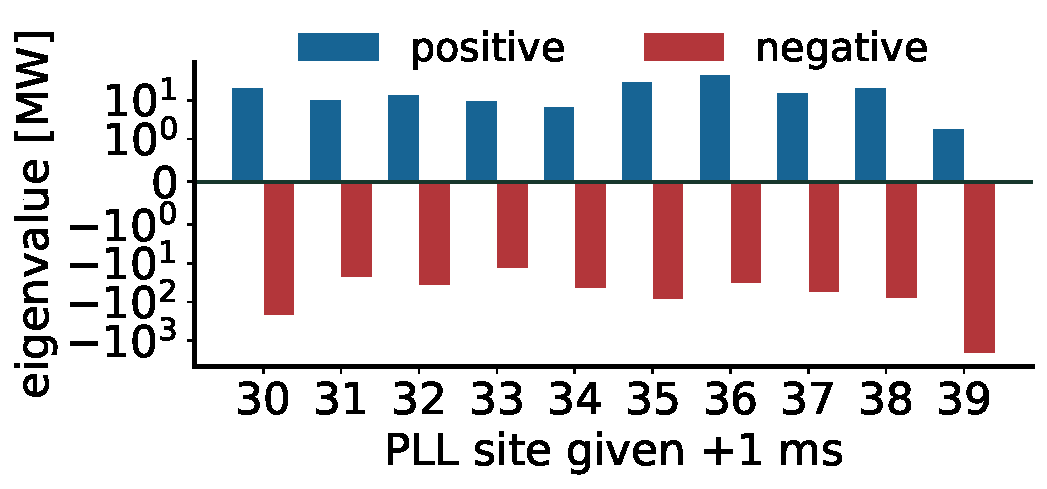
\includegraphics[width=148mm,height=78mm,keepaspectratio]{generated/figures/rank_two2.pdf}
  \end{minipage}\hfill%
  \begin{minipage}[c]{122mm}\raggedright
    {\DenseSmall IEEE-39, +1 ms at each PLL, 5 Hz: 60 of 60 checks, error $<5\times10^{-8}$.\par}\vspace{1.5mm}
    {\DenseSmall One frozen design: nodal term $+38.7$, collective term $-737.5$.\par}
  \end{minipage}\par
  \vspace{1.5mm}
  \begin{DenseWords}\textbf{\color{IASGold!65!black}COUNTING LAW\ \ }Removing $r$ anti-damped directions needs at least $r$ retuned PLLs, for any gain size (nine-bus bank at 8 Hz: $r=3$, interval-certified). Positive damping at one frequency is not stability.\end{DenseWords}
\end{DensePanel}
